\documentclass[11pt,a4paper]{article}
\usepackage[T1]{fontenc}
\usepackage[utf8]{inputenc}
\usepackage[margin=2.2cm]{geometry}
\usepackage{amsmath,amssymb,bm}
\usepackage{booktabs}
\usepackage{graphicx}
\usepackage{caption}
\usepackage{float}
\usepackage{array}
\usepackage{xcolor}
\usepackage[hidelinks]{hyperref}
\usepackage{tikz}
\usetikzlibrary{positioning, fit, calc, arrows.meta, backgrounds}
\pgfdeclarelayer{background}\pgfsetlayers{background,main}
\definecolor{inputgreen}{HTML}{C8E6C9}
\definecolor{processblue}{HTML}{BBDEFB}
\definecolor{metricgray}{HTML}{E0E0E0}
\definecolor{outputorange}{HTML}{FFE0B2}
\definecolor{midpurple}{HTML}{D1C4E9}
\definecolor{arrowgray}{HTML}{616161}
\definecolor{frozenslate}{HTML}{CFD8DC}
\newcommand{\best}[1]{\textbf{#1}}
\newcommand{\warn}[1]{\textcolor{red!70!black}{#1}}

\title{Coupling a conditional DDPM to its inverse model:\\
       four architectures under one protocol}
\author{}
\date{\today}

\begin{document}
\maketitle

\begin{abstract}
Four ways of relating a conditional DDPM to a pretrained Xception regressor are
evaluated on a single protocol: no coupling, a latent cosine term with the encoder
frozen, the same term with both networks trained, and sampling-time latent guidance.
Every variant is scored on three axes --- physical observables, parameter recovery
and sample diversity. Latent guidance raises the cycle $R^{2}$ from $0.639$ to
$0.915$ without reducing diversity, but a control experiment shows that most of
that gain is \emph{transported} by the guidance target rather than read from the
image, and that the physical observables do not improve. The cosine fine-tune buys
$+0.010$ in cycle $R^{2}$ and costs physical fidelity; trained jointly without an
anchor it collapses outright.
\end{abstract}

\section{Architectures}

All four share the same conditional DDPM ($g_\psi:\mathbb{R}^{8}\!\to\!\mathbb{R}^{39\times39}$)
and the same pretrained Xception regressor ($f_\phi:\mathbb{R}^{39\times39}\!\to\!\mathbb{R}^{8}$).
They differ only in how, and whether, gradients pass between them.

\begin{description}
  \item[(a) Baseline DDPM.] No coupling. The regressor only measures.
  \item[(b) Cosine loss, frozen encoder.] Training adds
        $\lambda_{\cos}\bigl(1-\cos(\mathbf{z}(\hat{\mathbf{x}}_0),\mathbf{z}(\mathbf{x}_0))\bigr)$,
        restricted to $t<t_{\max}$. Gradients traverse the frozen encoder and update
        the DDPM only.
  \item[(c) Cosine loss, joint fine-tune.] The encoder trains too. Both cosine
        branches then read the \emph{same} trainable encoder, so mapping every image
        to one direction makes $\cos\equiv1$ and the term vanishes. An inverse-regression
        anchor $\lambda_{\mathrm{inv}}\lVert f_\phi(\mathbf{X})-\bm{\theta}\rVert^{2}$
        makes that collapse expensive.
  \item[(d) Latent guidance.] No weight changes anywhere. A small network predicts a
        target latent $\mathbf{z}^{\star}=h(\bm{\theta})$, and each sampling step with
        $t<t_{\max}$ nudges the noise prediction,
        $\hat{\bm\epsilon}\leftarrow\hat{\bm\epsilon}
         +s\sqrt{1-\bar\alpha_t}\,\nabla_{\mathbf{x}_t}(1-\cos)/\lVert\nabla\rVert$.
\end{description}

\begin{figure}[htbp]
  \centering
  \resizebox{\textwidth}{!}{% =============================================================================
%  architectures.tex -- the four evaluated architectures on one comparison axis
%
%  Requires, in the preamble:
%    \usepackage{tikz}
%    \usetikzlibrary{positioning, fit, calc, arrows.meta, backgrounds}
%    \pgfdeclarelayer{background}\pgfsetlayers{background,main}
%    \definecolor{inputgreen}{HTML}{C8E6C9}
%    \definecolor{processblue}{HTML}{BBDEFB}
%    \definecolor{metricgray}{HTML}{E0E0E0}
%    \definecolor{outputorange}{HTML}{FFE0B2}
%    \definecolor{midpurple}{HTML}{D1C4E9}
%    \definecolor{arrowgray}{HTML}{616161}
%    \definecolor{frozenslate}{HTML}{CFD8DC}
%
%  Every variant is scored on the SAME three axes -- physical observables,
%  parameter recovery and diversity -- under one protocol, so the four rows of
%  the results table are comparable by construction.
% =============================================================================
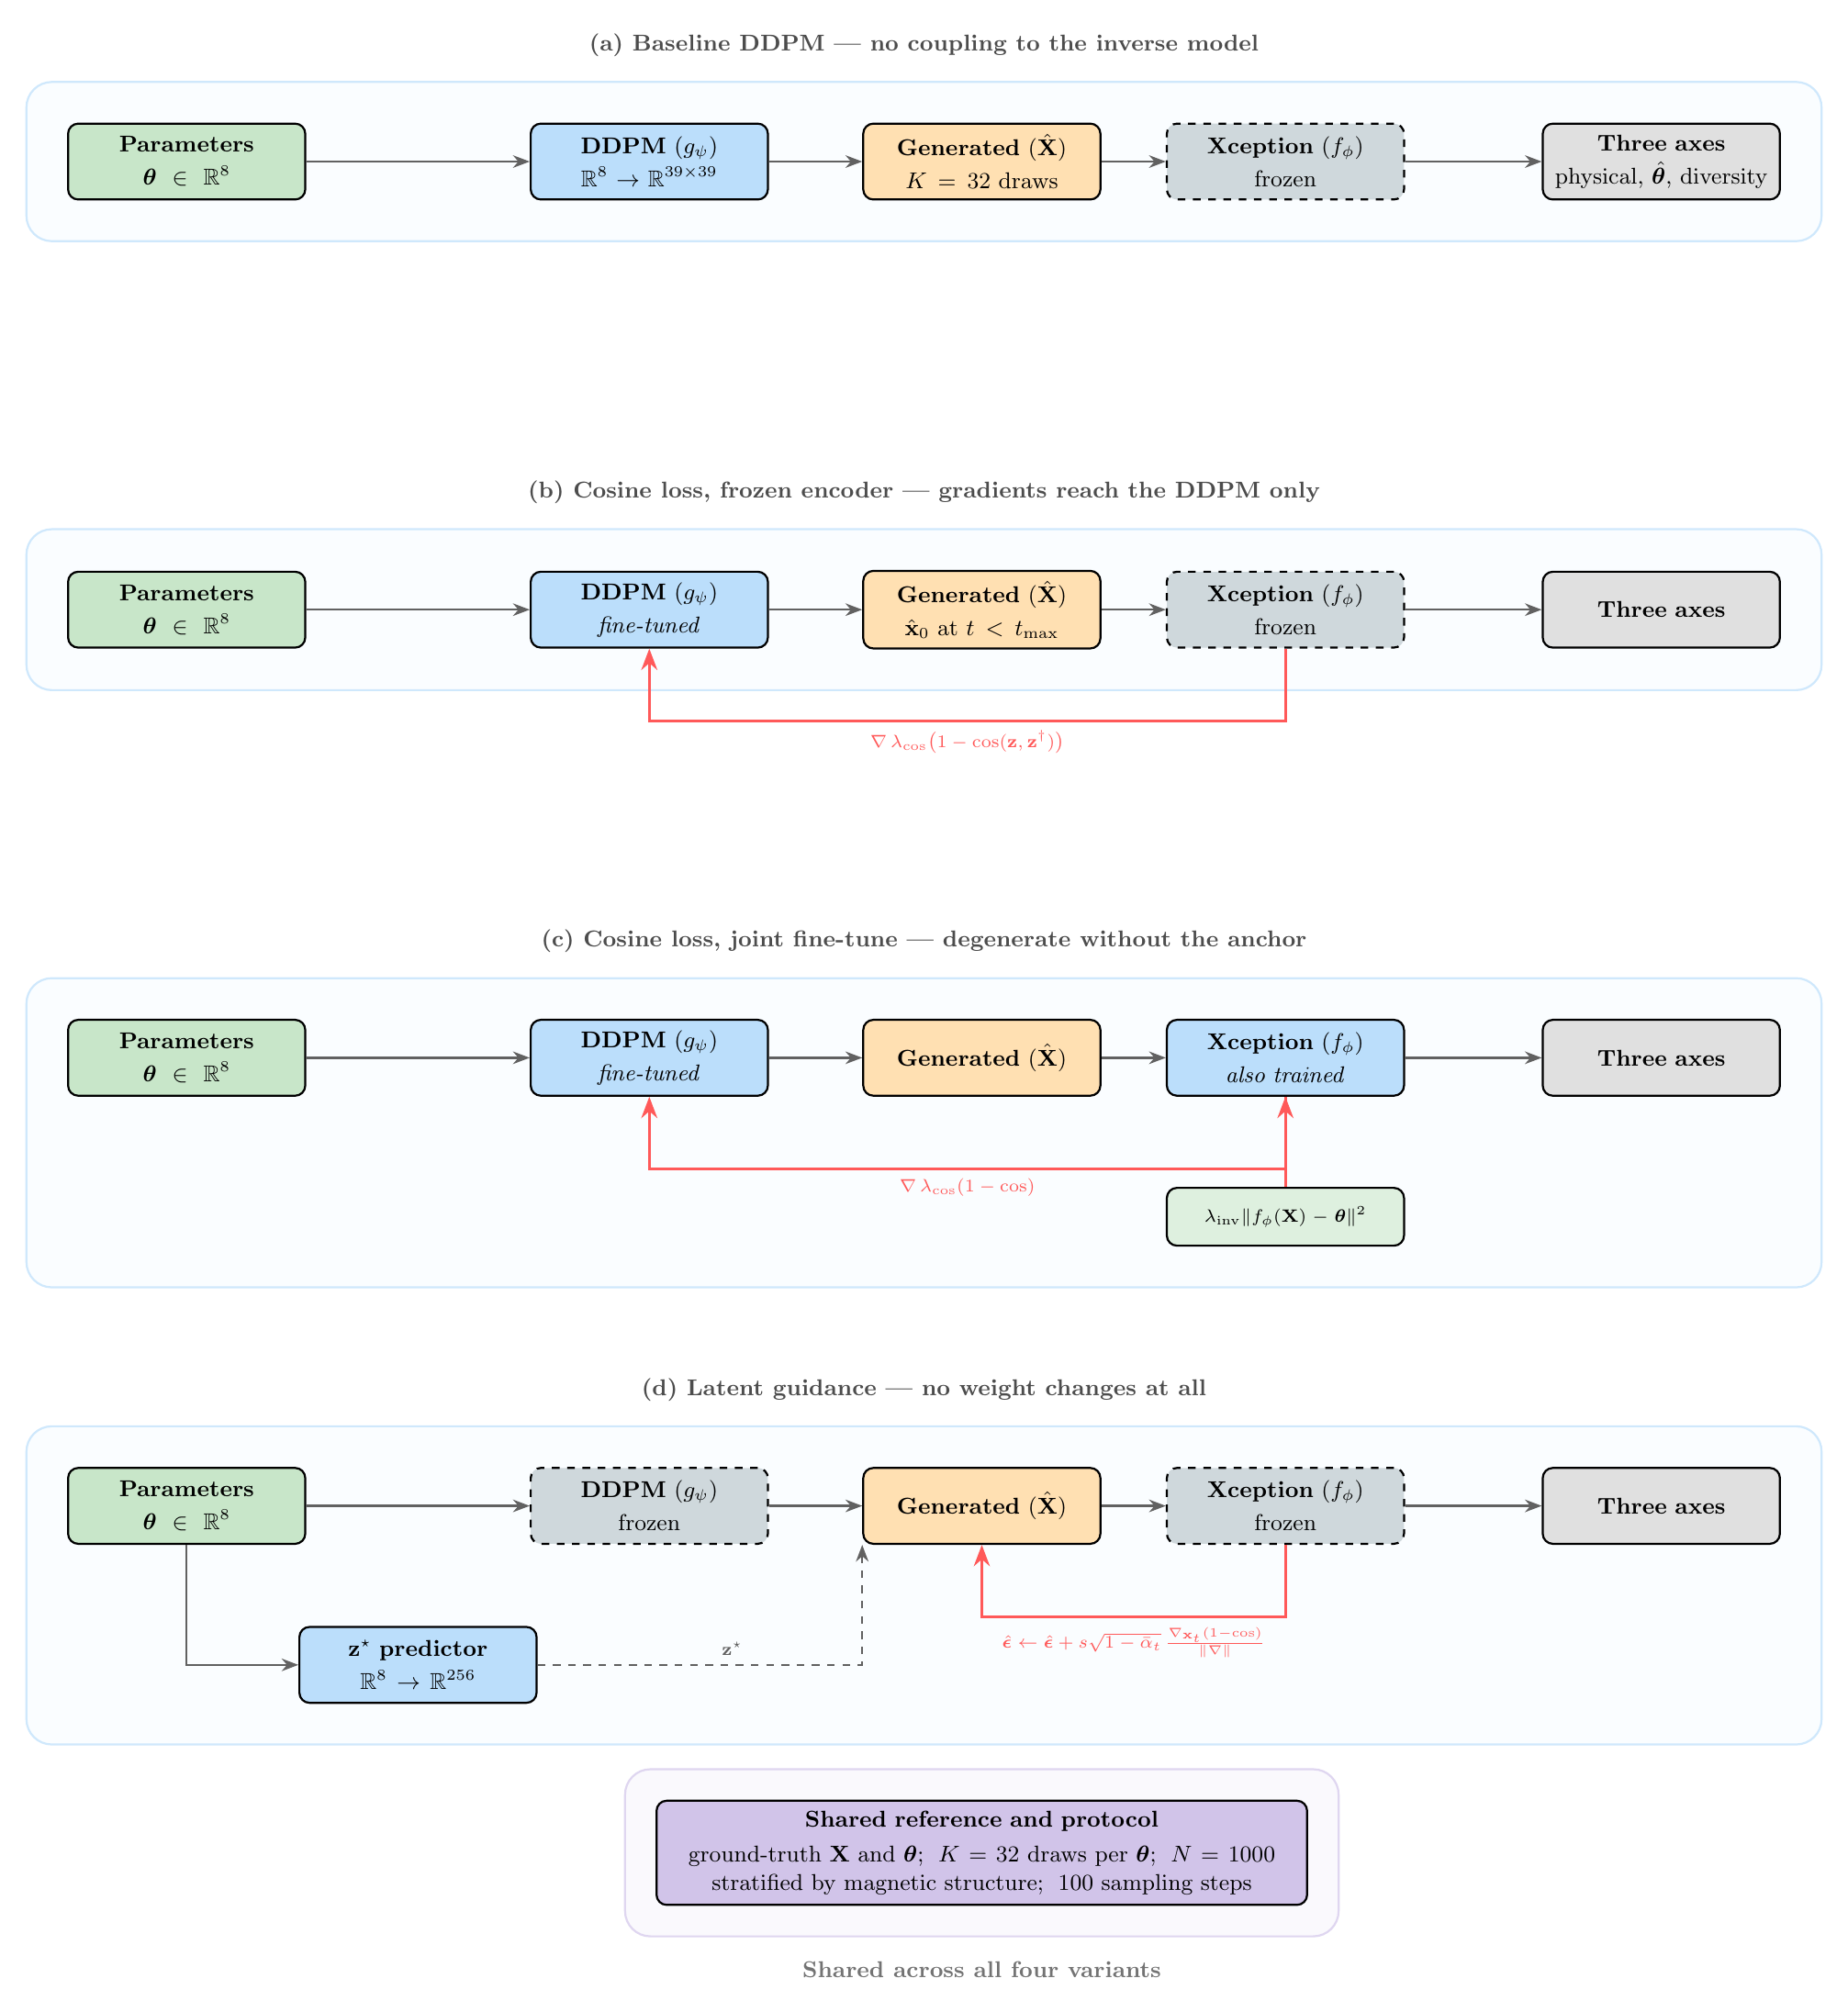
\begin{tikzpicture}[
  basebox/.style={draw, thick, rounded corners=4pt, minimum width=3.2cm, minimum height=1.05cm, text width=3.0cm, align=center, font=\small, inner sep=4pt},
  inputbox/.style={basebox, fill=inputgreen},
  modelbox/.style={basebox, fill=processblue},
  metricbox/.style={basebox, fill=metricgray},
  imgbox/.style={basebox, fill=outputorange},
  refbox/.style={basebox, fill=midpurple},
  frozenbox/.style={basebox, fill=frozenslate, dashed},
  arr/.style={thick, ->, >=Stealth, color=arrowgray},
  darr/.style={thick, ->, >=Stealth, color=arrowgray, dashed},
  gradarr/.style={very thick, ->, >=Stealth, color=red!65},
  lbl/.style={font=\scriptsize\itshape, color=arrowgray},
  seclbl/.style={font=\small\bfseries, color=black!55},
  vlbl/.style={font=\small\bfseries, color=black!70}
]

% =============================================================================
%  Layout
%  Col1=0  |  Col2=6.4  |  Col3=11.0  |  Col4=15.2  |  Col5=20.4
%  Row A=0 (base)  |  Row B=-6.2 (frozen)  |  Row C=-12.4 (joint)  |  Row D=-18.6 (guided)
% =============================================================================

% ══ VARIANT A -- baseline DDPM ══════════════════════════════════════════════
\node[inputbox]  (Atheta) at (0, 0)    {\textbf{Parameters}\\[2pt]$\boldsymbol{\theta}\in\mathbb{R}^{8}$};
\node[modelbox]  (Agm)    at (6.4, 0)  {\textbf{DDPM} ($g_\psi$)\\[2pt]$\mathbb{R}^{8}\!\to\!\mathbb{R}^{39\times39}$};
\node[imgbox]    (Axhat)  at (11.0, 0) {\textbf{Generated} ($\hat{\mathbf{X}}$)\\[2pt]$K=32$ draws};
\node[frozenbox] (Aim)    at (15.2, 0) {\textbf{Xception} ($f_\phi$)\\[2pt]frozen};
\node[metricbox] (Amet)   at (20.4, 0) {\textbf{Three axes}\\[2pt]physical, $\hat{\boldsymbol{\theta}}$, diversity};

\draw[arr] (Atheta.east) -- (Agm.west);
\draw[arr] (Agm.east)    -- (Axhat.west);
\draw[arr] (Axhat.east)  -- (Aim.west);
\draw[arr] (Aim.east)    -- (Amet.west);

% ══ VARIANT B -- cosine loss, frozen encoder ════════════════════════════════
\node[inputbox]  (Btheta) at (0, -6.2)    {\textbf{Parameters}\\[2pt]$\boldsymbol{\theta}\in\mathbb{R}^{8}$};
\node[modelbox]  (Bgm)    at (6.4, -6.2)  {\textbf{DDPM} ($g_\psi$)\\[2pt]\emph{fine-tuned}};
\node[imgbox]    (Bxhat)  at (11.0, -6.2) {\textbf{Generated} ($\hat{\mathbf{X}}$)\\[2pt]$\hat{\mathbf{x}}_0$ at $t<t_{\max}$};
\node[frozenbox] (Bim)    at (15.2, -6.2) {\textbf{Xception} ($f_\phi$)\\[2pt]frozen};
\node[metricbox] (Bmet)   at (20.4, -6.2) {\textbf{Three axes}};

\draw[arr] (Btheta.east) -- (Bgm.west);
\draw[arr] (Bgm.east)    -- (Bxhat.west);
\draw[arr] (Bxhat.east)  -- (Bim.west);
\draw[arr] (Bim.east)    -- (Bmet.west);
% cosine gradient flows back through the frozen encoder into the DDPM
\draw[gradarr] (Bim.south) -- ++(0,-1.0) -| (Bgm.south)
  node[lbl, pos=0.25, below, color=red!65] {$\nabla\,\lambda_{\cos}\bigl(1-\cos(\mathbf{z},\mathbf{z}^{\dagger})\bigr)$};

% ══ VARIANT C -- cosine loss, joint fine-tune ═══════════════════════════════
\node[inputbox]  (Ctheta) at (0, -12.4)    {\textbf{Parameters}\\[2pt]$\boldsymbol{\theta}\in\mathbb{R}^{8}$};
\node[modelbox]  (Cgm)    at (6.4, -12.4)  {\textbf{DDPM} ($g_\psi$)\\[2pt]\emph{fine-tuned}};
\node[imgbox]    (Cxhat)  at (11.0, -12.4) {\textbf{Generated} ($\hat{\mathbf{X}}$)};
\node[modelbox]  (Cim)    at (15.2, -12.4) {\textbf{Xception} ($f_\phi$)\\[2pt]\emph{also trained}};
\node[metricbox] (Cmet)   at (20.4, -12.4) {\textbf{Three axes}};

\draw[arr] (Ctheta.east) -- (Cgm.west);
\draw[arr] (Cgm.east)    -- (Cxhat.west);
\draw[arr] (Cxhat.east)  -- (Cim.west);
\draw[arr] (Cim.east)    -- (Cmet.west);
\draw[gradarr] (Cim.south) -- ++(0,-1.0) -| (Cgm.south)
  node[lbl, pos=0.25, below, color=red!65] {$\nabla\,\lambda_{\cos}(1-\cos)$};
% the anchor that makes the joint objective well-posed
\node[metricbox, fill=inputgreen!60, minimum height=0.8cm] (Canchor) at (15.2, -14.6)
  {\scriptsize$\lambda_{\mathrm{inv}}\lVert f_\phi(\mathbf{X})-\boldsymbol{\theta}\rVert^{2}$};
\draw[gradarr] (Canchor.north) -- (Cim.south);

% ══ VARIANT D -- latent guidance at sampling time ═══════════════════════════
\node[inputbox]  (Dtheta) at (0, -18.6)    {\textbf{Parameters}\\[2pt]$\boldsymbol{\theta}\in\mathbb{R}^{8}$};
\node[modelbox]  (Dpred)  at (3.2, -20.8)  {\textbf{$\mathbf{z}^{\star}$ predictor}\\[2pt]$\mathbb{R}^{8}\!\to\!\mathbb{R}^{256}$};
\node[frozenbox] (Dgm)    at (6.4, -18.6)  {\textbf{DDPM} ($g_\psi$)\\[2pt]frozen};
\node[imgbox]    (Dxhat)  at (11.0, -18.6) {\textbf{Generated} ($\hat{\mathbf{X}}$)};
\node[frozenbox] (Dim)    at (15.2, -18.6) {\textbf{Xception} ($f_\phi$)\\[2pt]frozen};
\node[metricbox] (Dmet)   at (20.4, -18.6) {\textbf{Three axes}};

\draw[arr] (Dtheta.east) -- (Dgm.west);
\draw[arr] (Dtheta.south) |- (Dpred.west);
\draw[arr] (Dgm.east)    -- (Dxhat.west);
\draw[arr] (Dxhat.east)  -- (Dim.west);
\draw[arr] (Dim.east)    -- (Dmet.west);
% per-step guidance: nudges the noise prediction, changes no weight
\draw[gradarr] (Dim.south) -- ++(0,-1.0) -| (Dxhat.south)
  node[lbl, pos=0.25, below, color=red!65] {$\hat{\boldsymbol{\epsilon}}\leftarrow\hat{\boldsymbol{\epsilon}}+s\sqrt{1-\bar{\alpha}_t}\,\frac{\nabla_{\mathbf{x}_t}(1-\cos)}{\lVert\nabla\rVert}$};
\draw[darr] (Dpred.east) -| (Dxhat.south west)
  node[lbl, pos=0.3, above] {$\mathbf{z}^{\star}$};

% ══ SHARED REFERENCE COLUMN ════════════════════════════════════════════════
% Placed once, below the four variants. Deliberately NOT wired with arrows: a
% connector to each of the four metric boxes draws a vertical line straight through
% every panel and makes the figure unreadable. The shared inputs are stated in the
% label instead.
\node[refbox, minimum width=9cm, text width=8.6cm] (ref) at (11.0, -23.4)
  {\textbf{Shared reference and protocol}\\[3pt]
   ground-truth $\mathbf{X}$ and $\boldsymbol{\theta}$;\;
   $K=32$ draws per $\boldsymbol{\theta}$;\;
   $N=1000$ stratified by magnetic structure;\;
   $100$ sampling steps};

% =============================================================================
%  BACKGROUND PANELS
% =============================================================================
\begin{pgfonlayer}{background}
  \node[draw=processblue!70, fill=processblue!7, rounded corners=10pt, thick,
        fit=(Atheta)(Agm)(Axhat)(Aim)(Amet), inner sep=16pt] (panelA) {};
  \node[draw=processblue!70, fill=processblue!7, rounded corners=10pt, thick,
        fit=(Btheta)(Bgm)(Bxhat)(Bim)(Bmet), inner sep=16pt] (panelB) {};
  \node[draw=processblue!70, fill=processblue!7, rounded corners=10pt, thick,
        fit=(Ctheta)(Cgm)(Cxhat)(Cim)(Cmet)(Canchor), inner sep=16pt] (panelC) {};
  \node[draw=processblue!70, fill=processblue!7, rounded corners=10pt, thick,
        fit=(Dtheta)(Dpred)(Dgm)(Dxhat)(Dim)(Dmet), inner sep=16pt] (panelD) {};
  \node[draw=midpurple!70, fill=midpurple!10, rounded corners=10pt, thick,
        fit=(ref), inner sep=12pt] (panelR) {};
\end{pgfonlayer}

\node[vlbl, above=6pt of panelA] {(a) Baseline DDPM --- no coupling to the inverse model};
\node[vlbl, above=6pt of panelB] {(b) Cosine loss, frozen encoder --- gradients reach the DDPM only};
\node[vlbl, above=6pt of panelC] {(c) Cosine loss, joint fine-tune --- degenerate without the anchor};
\node[vlbl, above=6pt of panelD] {(d) Latent guidance --- no weight changes at all};
\node[seclbl, below=6pt of panelR] {Shared across all four variants};

\end{tikzpicture}
}
  \caption{The four variants. Red paths mark what each one couples: nothing for the
  baseline, the DDPM only for the frozen-encoder cosine, both networks plus the anchor
  for the joint variant, and a per-step nudge that changes no weight for guidance.}
\end{figure}

\section{Protocol}

A conditional DDPM draws a \emph{realisation} of $p(\mathbf{x}\mid\bm\theta)$, so scoring a
single draw against a single reference caps $R^{2}$ at the intrinsic conditional
variance even for a perfect model. Every number below therefore averages $K=32$ draws
per $\bm\theta$ before scoring. The predicted parameters are averaged the same way ---
each realisation is encoded and the eight outputs averaged; the \emph{images} are never
averaged, which would produce a non-physical mean texture.

\begin{center}\small
\begin{tabular}{ll}
\toprule
Draws per $\bm\theta$ & $K=32$ \\
Conditioning points & $N=1000$, sampled proportionally by magnetic structure \\
Sampling steps & $100$ \\
Seed & $42$, identical across variants \\
\bottomrule
\end{tabular}
\end{center}

\section{Physical observables}

\begin{table}[htbp]
\centering
\caption{Agreement between generated and reference observables, $R^{2}$ of the
conditional mean over $K$ draws. Higher is better.}
\begin{tabular}{lcccc}
\toprule
Model & $M$ & $C_{nn}$ & $q_{\mathrm{peak}}$ & SSIM \\
\midrule
DDPM base            & \best{0.7954} & 0.8521        & 0.5924        & \best{0.1753} \\
$+$ cos (frozen)     & 0.7886        & 0.8292        & 0.5046        & 0.1591 \\
$+$ cos (joint)      & \multicolumn{4}{c}{\warn{collapsed --- see Section~\ref{sec:collapse}}} \\
$+$ guidance ($s=8$) & 0.7775        & \best{0.8602} & \best{0.6060} & 0.1713 \\
\bottomrule
\end{tabular}
\end{table}

No variant improves on the baseline overall. Guidance is marginally better on
$C_{nn}$ and $q_{\mathrm{peak}}$ and slightly worse on $M$; the cosine fine-tune is
worse on all three.

\paragraph{A caution on $q_{\mathrm{peak}}$.}
The value above is the \emph{masked, mean-subtracted} peak wavevector: the structure
factor is computed on the nanodot disk with the disk mean removed, and reported in
rad per lattice site. Earlier comparison notebooks call the same routine with its
default arguments --- raw image, no disk mask, no mean removed --- and report the raw
radial bin. Those are different quantities and their $q_{\mathrm{peak}}$ columns must
never be placed side by side.

\section{Parameter recovery}

\begin{table}[htbp]
\centering
\caption{Cycle $R^{2}$: $\bm\theta\to$ DDPM $\to f_\phi\to\hat{\bm\theta}$, per parameter.
The last column is the control of Section~\ref{sec:control}. Here $h$ is the network that
predicts the guidance target, $\mathbf{z}^{\star}=h(\bm\theta)$, and \emph{head} is the final
regression stage of $f_\phi$, which maps a 256-dimensional latent to the eight parameters.
The column is $\mathrm{head}(h(\bm\theta))$: the target latent fed straight into the head,
so the path is $\bm\theta\to\mathbb{R}^{256}\to\hat{\bm\theta}$ and \textbf{no image is ever
generated or encoded}.}
\begin{tabular}{lcccc}
\toprule
& DDPM base & $+$ cos (frozen) & $+$ guidance & \warn{\shortstack{control:\\$\mathrm{head}(h(\bm\theta))$\\no image}} \\
\midrule
$T^{(0)}$        & 0.9636 & 0.9436 & \best{0.9924} & 0.9956 \\
$\tilde{J}_{2}$  & 0.9256 & 0.7496 & \best{0.9675} & 0.9905 \\
$\tilde{J}_{3}$  & 0.0060 & $-$0.0028 & \best{0.7996} & \warn{0.8790} \\
$\tilde{J}_{4}$  & $-$0.0118 & $-$0.0205 & \best{0.7967} & \warn{0.8665} \\
$\tilde{K}_{\mathrm{an}1}$ & 0.6076 & 0.7353 & \best{0.8844} & 0.9705 \\
$\tilde{K}_{\mathrm{an}S}$ & 0.7865 & 0.8314 & \best{0.9655} & 0.9852 \\
$\tilde{H}_{\mathrm{ex}}$  & 0.8375 & \best{0.9583} & 0.9175 & 0.9928 \\
$\tilde{K}_{\mathrm{DM}}$  & 0.9946 & 0.9954 & \best{0.9964} & 0.9965 \\
\midrule
\textbf{mean}    & 0.6387 & 0.6488 & \best{0.9150} & \warn{0.9596} \\
\bottomrule
\end{tabular}
\end{table}

The cosine fine-tune moves the mean by $+0.010$, which is within noise. Guidance moves
it by $+0.276$, and almost all of that comes from $\tilde{J}_{3}$ and $\tilde{J}_{4}$
rising from zero to about $0.80$.

\section{Control: where does that gain come from?}\label{sec:control}

$\tilde{J}_{3}$ and $\tilde{J}_{4}$ are the two parameters the predecessor work reports
as unidentifiable from the $s_z$ projection. Our own measurement agrees: applied to
\emph{real simulated configurations}, the regressor scores $-0.1125$ and $-0.2467$ on
them. No real configuration reaches $0.80$.

Composing the guidance target with the regression head, $\mathrm{head}(h(\bm\theta))$,
and evaluating it on the test parameters \emph{without generating any image} gives
$0.8790$ and $0.8665$ on those same two parameters, and a mean of $0.9596$. Guidance
scores $0.9150$ --- just below, approaching from underneath.

That composition is an autoencoder of $\bm\theta$ through a 256-dimensional bottleneck
that never touches an image. Guidance transports $\bm\theta$ along it, using the image
as a lossy channel. Two mechanisms are therefore mixed, and they separate by parameter:

\begin{itemize}
  \item \emph{Legitimate.} For identifiable parameters, guidance steers the draw toward
        the typical region of $p(\mathbf{x}\mid\bm\theta)$ and shrinks the stochastic
        dispersion that hurts recovery ($T^{(0)}$: $0.964\to0.992$).
  \item \emph{Circular.} For $\tilde{J}_{3}$ and $\tilde{J}_{4}$ there is no information
        in the image to sharpen, so $0.006\to0.800$ can only be transported.
\end{itemize}

This does \emph{not} contradict the identifiability claim of the predecessor work. That
claim concerns real configurations, and our measurement confirms it. Guided images are
not samples of $p(\mathbf{x}\mid\bm\theta)$; they are constructed to carry a target
latent, and their physical observables do not improve. The value $0.9596$ is a ceiling
on what latent guidance can ever score on this metric --- set by the predictor and the
head, not by the physics.

\section{Diversity}

Averaging $K$ draws hides a collapse: identical draws average to a clean value. The
Vendi score reports the effective number of distinct draws per $\bm\theta$, from $1$
(collapsed) to $K=32$ (fully diverse).

\begin{table}[htbp]
\centering
\caption{Diversity of the $K$ draws of one $\bm\theta$. The reference is the same score
over the $K$ nearest real neighbours in parameter space --- a loose upper bound, not a
target, since neighbours differ in $\bm\theta$ and so vary for reasons beyond sampling.}
\begin{tabular}{lcc}
\toprule
Model & Vendi (pixels) & Vendi (latent) \\
\midrule
DDPM base            & 13.29 & 1.51 \\
$+$ cos (frozen)     & \best{14.22} & 1.43 \\
$+$ guidance ($s=8$) & 13.26 & 1.09 \\
\midrule
real neighbours (ref)& 13.70 & --- \\
\bottomrule
\end{tabular}
\end{table}

No variant loses generative stochasticity: pixel diversity stays near the reference in
every case. The latent Vendi is low throughout, and means opposite things depending on
the variant. For a frozen encoder a value near $1$ is \emph{correct} --- the encoder is
meant to be invariant to which realisation it sees and to report only $\bm\theta$. When
the encoder is trained, the same number is degeneracy. Latent Vendi must therefore be
read next to the inverse-model $R^{2}$, never alone.

\section{Joint fine-tuning collapses}\label{sec:collapse}

Trained without the anchor, the joint variant found the degenerate solution within one
epoch. The cosine term reached $0.0000$ by epoch~3 --- satisfied trivially, contributing
no gradient --- while the encoder's held-out $R^{2}$ went negative immediately and
reached $-114{,}134$ by epoch~14, ending at a cycle $R^{2}$ of $-146{,}409$.

Its \emph{physical} metrics ($0.7496$, $0.8456$, $0.6838$) look better than the
frozen-encoder variant's. They are not a success: once the cosine gradient vanished the
DDPM was left almost untouched. Reporting them as a win would invert the finding.

\section{Generated textures}

\begin{figure}[H]
  \centering
  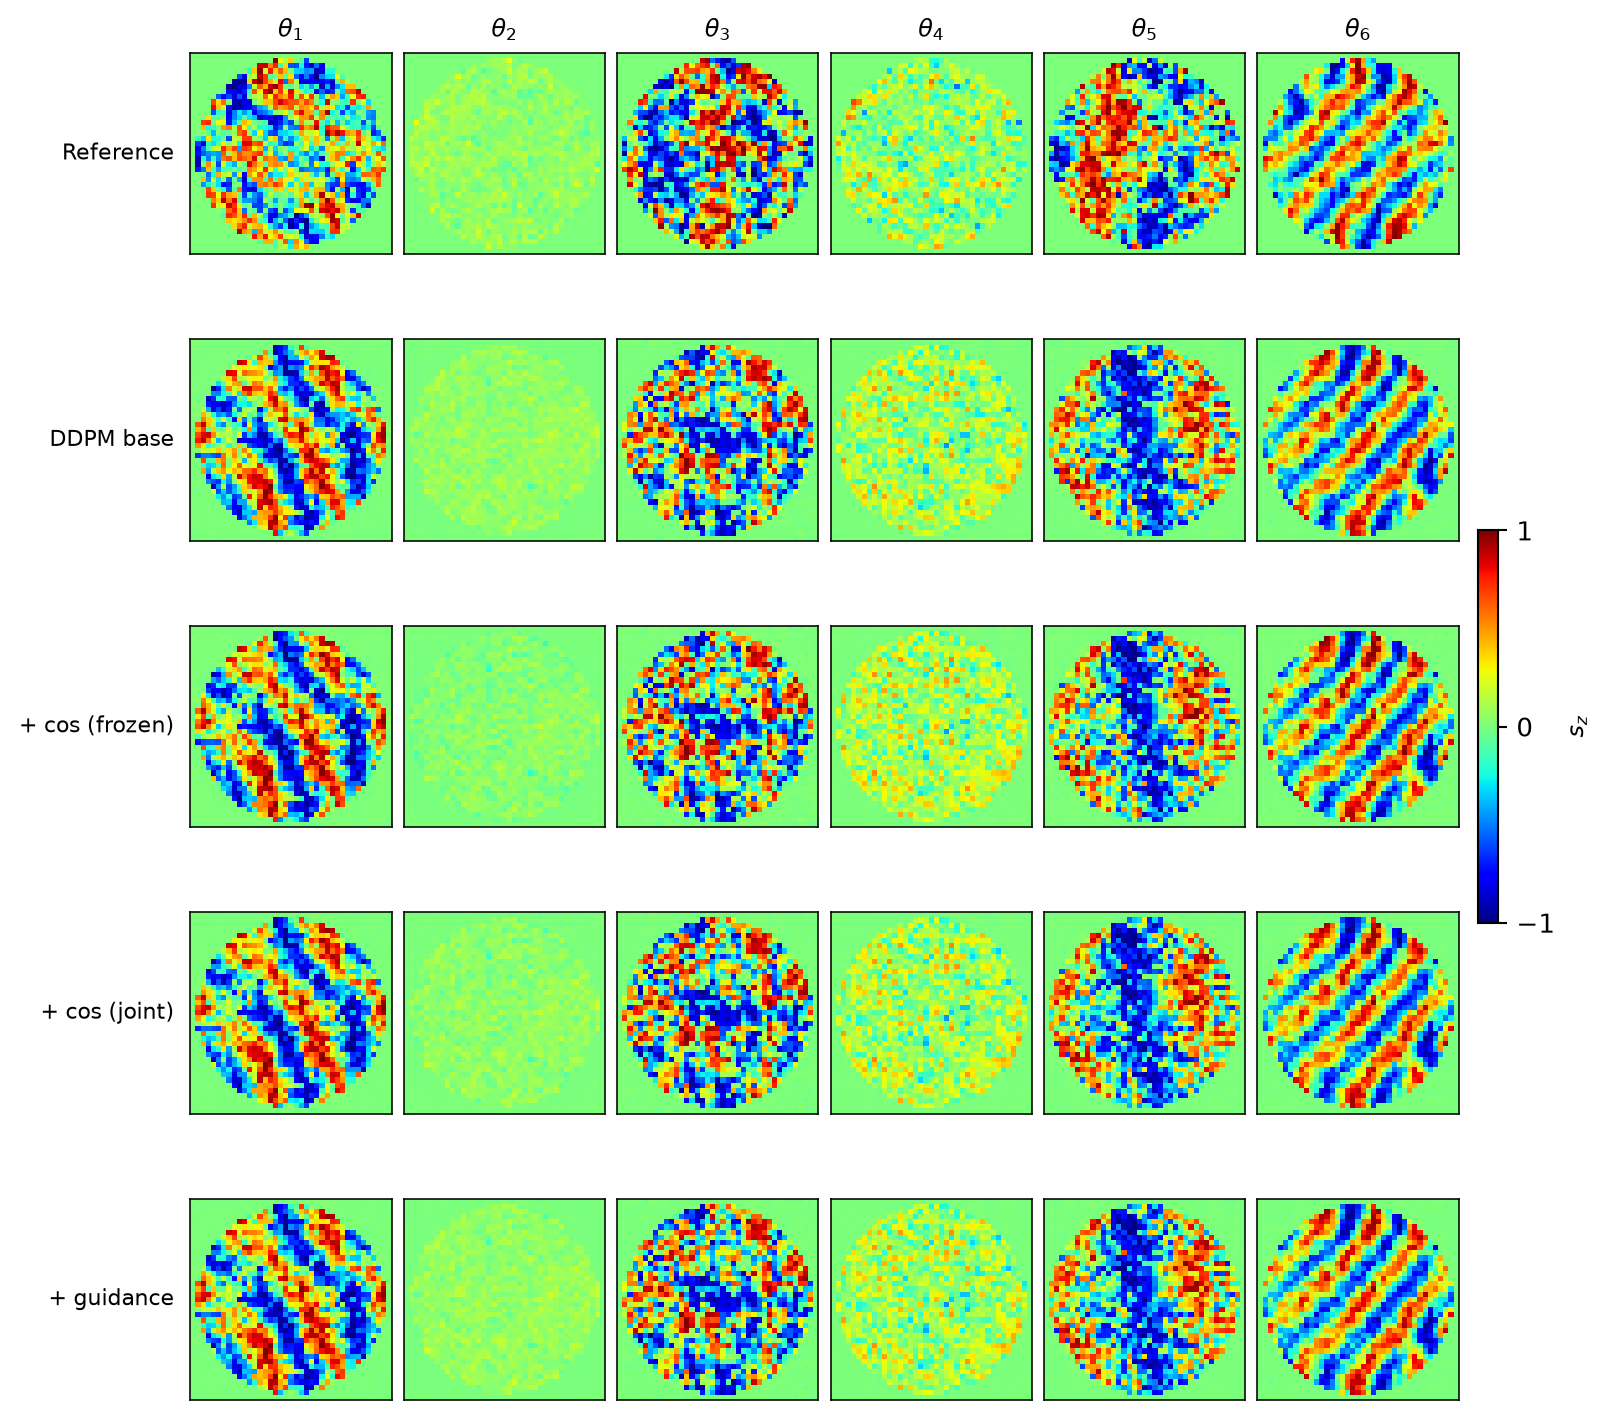
\includegraphics[width=\textwidth]{grid.png}
  \caption{Central-layer $s_z$ projections. Top row: the reference simulated
  configuration. Below, one draw from each variant for the \emph{same} $\bm\theta$, same
  seed, same sampling steps. Colour map \texttt{jet} with the scale pinned to $[-1,1]$ in every panel, so $s_z=0$ always renders as the same green and colours are comparable across models and across $\bm\theta$.}
\end{figure}

\section{Summary}

\begin{center}\small
\begin{tabular}{lccc}
\toprule
& Physical observables & Parameter recovery & Diversity \\
\midrule
$+$ cos (frozen) & worse & $+0.010$ (noise) & preserved \\
$+$ cos (joint)  & \warn{collapsed} & \warn{collapsed} & \warn{collapsed} \\
$+$ guidance     & unchanged & $+0.276$, mostly transported & preserved \\
\bottomrule
\end{tabular}
\end{center}

The defensible claim is narrow: latent guidance markedly improves the cycle metric at no
cost in diversity and none in physical fidelity, while a control shows that most of the
improvement does not come from the image. Coupling through a training loss, in either
form tried here, does not pay for itself.

\end{document}
